
\documentclass[a4paper,11pt]{article}
\usepackage[a4paper, margin=8em]{geometry}

% usa i pacchetti per la scrittura in italiano
\usepackage[french,italian]{babel}
\usepackage[T1]{fontenc}
\usepackage[utf8]{inputenc}
\frenchspacing 

% usa i pacchetti per la formattazione matematica
\usepackage{amsmath, amssymb, amsthm, amsfonts}

% usa altri pacchetti
\usepackage{gensymb}
\usepackage{hyperref}
\usepackage{standalone}

\usepackage{colortbl}

\usepackage{xstring}
\usepackage{karnaugh-map}

% imposta il titolo
\title{Appunti Calcolatori Elettronici}
\author{Luca Seggiani}
\date{2025}

% imposta lo stile
% usa helvetica
\usepackage[scaled]{helvet}
% usa palatino
\usepackage{palatino}
% usa un font monospazio guardabile
\usepackage{lmodern}

\renewcommand{\rmdefault}{ppl}
\renewcommand{\sfdefault}{phv}
\renewcommand{\ttdefault}{lmtt}

% circuiti
\usepackage{circuitikz}
\usetikzlibrary{babel}

% testo cerchiato
\newcommand*\circled[1]{\tikz[baseline=(char.base)]{
            \node[shape=circle,draw,inner sep=2pt] (char) {#1};}}

% disponi il titolo
\makeatletter
\renewcommand{\maketitle} {
	\begin{center} 
		\begin{minipage}[t]{.8\textwidth}
			\textsf{\huge\bfseries \@title} 
		\end{minipage}%
		\begin{minipage}[t]{.2\textwidth}
			\raggedleft \vspace{-1.65em}
			\textsf{\small \@author} \vfill
			\textsf{\small \@date}
		\end{minipage}
		\par
	\end{center}

	\thispagestyle{empty}
	\pagestyle{fancy}
}
\makeatother

% disponi teoremi
\usepackage{tcolorbox}
\newtcolorbox[auto counter, number within=section]{theorem}[2][]{%
	colback=blue!10, 
	colframe=blue!40!black, 
	sharp corners=northwest,
	fonttitle=\sffamily\bfseries, 
	title=Teorema~\thetcbcounter: #2, 
	#1
}

% disponi definizioni
\newtcolorbox[auto counter, number within=section]{definition}[2][]{%
	colback=red!10,
	colframe=red!40!black,
	sharp corners=northwest,
	fonttitle=\sffamily\bfseries,
	title=Definizione~\thetcbcounter: #2,
	#1
}

% disponi codice
\usepackage{listings}
\usepackage[table]{xcolor}

\definecolor{codegreen}{rgb}{0,0.6,0}
\definecolor{codegray}{rgb}{0.5,0.5,0.5}
\definecolor{codepurple}{rgb}{0.58,0,0.82}
\definecolor{backcolour}{rgb}{0.95,0.95,0.92}

\lstdefinestyle{codestyle}{
		backgroundcolor=\color{black!5}, 
		commentstyle=\color{codegreen},
		keywordstyle=\bfseries\color{magenta},
		numberstyle=\sffamily\tiny\color{black!60},
		stringstyle=\color{green!50!black},
		basicstyle=\ttfamily\footnotesize,
		breakatwhitespace=false,         
		breaklines=true,                 
		captionpos=b,                    
		keepspaces=true,                 
		numbers=left,                    
		numbersep=5pt,                  
		showspaces=false,                
		showstringspaces=false,
		showtabs=false,                  
		tabsize=2
}

\lstdefinestyle{shellstyle}{
		backgroundcolor=\color{black!5}, 
		basicstyle=\ttfamily\footnotesize\color{black}, 
		commentstyle=\color{black}, 
		keywordstyle=\color{black},
		numberstyle=\color{black!5},
		stringstyle=\color{black}, 
		showspaces=false,
		showstringspaces=false, 
		showtabs=false, 
		tabsize=2, 
		numbers=none, 
		breaklines=true
}


\lstdefinelanguage{assembler}{ 
  keywords={AAA, AAD, AAM, AAS, ADC, ADCB, ADCW, ADCL, ADD, ADDB, ADDW, ADDL, AND, ANDB, ANDW, ANDL,
        ARPL, BOUND, BSF, BSFL, BSFW, BSR, BSRL, BSRW, BSWAP, BT, BTC, BTCB, BTCW, BTCL, BTR, 
        BTRB, BTRW, BTRL, BTS, BTSB, BTSW, BTSL, CALL, CBW, CDQ, CLC, CLD, CLI, CLTS, CMC, CMP,
        CMPB, CMPW, CMPL, CMPS, CMPSB, CMPSD, CMPSW, CMPXCHG, CMPXCHGB, CMPXCHGW, CMPXCHGL,
        CMPXCHG8B, CPUID, CWDE, DAA, DAS, DEC, DECB, DECW, DECL, DIV, DIVB, DIVW, DIVL, ENTER,
        HLT, IDIV, IDIVB, IDIVW, IDIVL, IMUL, IMULB, IMULW, IMULL, IN, INB, INW, INL, INC, INCB,
        INCW, INCL, INS, INSB, INSD, INSW, INT, INT3, INTO, INVD, INVLPG, IRET, IRETD, JA, JAE,
        JB, JBE, JC, JCXZ, JE, JECXZ, JG, JGE, JL, JLE, JMP, JNA, JNAE, JNB, JNBE, JNC, JNE, JNG,
        JNGE, JNL, JNLE, JNO, JNP, JNS, JNZ, JO, JP, JPE, JPO, JS, JZ, LAHF, LAR, LCALL, LDS,
        LEA, LEAVE, LES, LFS, LGDT, LGS, LIDT, LMSW, LOCK, LODSB, LODSD, LODSW, LOOP, LOOPE,
        LOOPNE, LSL, LSS, LTR, MOV, MOVB, MOVW, MOVL, MOVSB, MOVSD, MOVSW, MOVSX, MOVSXB,
        MOVSXW, MOVSXL, MOVZX, MOVZXB, MOVZXW, MOVZXL, MUL, MULB, MULW, MULL, NEG, NEGB, NEGW,
        NEGL, NOP, NOT, NOTB, NOTW, NOTL, OR, ORB, ORW, ORL, OUT, OUTB, OUTW, OUTL, OUTSB, OUTSD,
        OUTSW, POP, POPL, POPW, POPB, POPA, POPAD, POPF, POPFD, PUSH, PUSHL, PUSHW, PUSHB, PUSHA, 
				PUSHAD, PUSHF, PUSHFD, RCL, RCLB, RCLW, MOVSL, MOVSB, MOVSW, STOSL, STOSB, STOSW, LODSB, LODSW,
				LODSL, INSB, INSW, INSL, OUTSB, OUTSL, OUTSW
        RCLL, RCR, RCRB, RCRW, RCRL, RDMSR, RDPMC, RDTSC, REP, REPE, REPNE, RET, ROL, ROLB, ROLW,
        ROLL, ROR, RORB, RORW, RORL, SAHF, SAL, SALB, SALW, SALL, SAR, SARB, SARW, SARL, SBB,
        SBBB, SBBW, SBBL, SCASB, SCASD, SCASW, SETA, SETAE, SETB, SETBE, SETC, SETE, SETG, SETGE,
        SETL, SETLE, SETNA, SETNAE, SETNB, SETNBE, SETNC, SETNE, SETNG, SETNGE, SETNL, SETNLE,
        SETNO, SETNP, SETNS, SETNZ, SETO, SETP, SETPE, SETPO, SETS, SETZ, SGDT, SHL, SHLB, SHLW,
        SHLL, SHLD, SHR, SHRB, SHRW, SHRL, SHRD, SIDT, SLDT, SMSW, STC, STD, STI, STOSB, STOSD,
        STOSW, STR, SUB, SUBB, SUBW, SUBL, TEST, TESTB, TESTW, TESTL, VERR, VERW, WAIT, WBINVD,
        XADD, XADDB, XADDW, XADDL, XCHG, XCHGB, XCHGW, XCHGL, XLAT, XLATB, XOR, XORB, XORW, XORL},
  keywordstyle=\color{blue}\bfseries,
  ndkeywordstyle=\color{darkgray}\bfseries,
  identifierstyle=\color{black},
  sensitive=false,
  comment=[l]{\#},
  morecomment=[s]{/*}{*/},
  commentstyle=\color{purple}\ttfamily,
  stringstyle=\color{red}\ttfamily,
  morestring=[b]',
  morestring=[b]"
}

\lstset{language=assembler, style=codestyle}

% disponi sezioni
\usepackage{titlesec}

\titleformat{\section}
	{\sffamily\Large\bfseries} 
	{\thesection}{1em}{} 
\titleformat{\subsection}
	{\sffamily\large\bfseries}   
	{\thesubsection}{1em}{} 
\titleformat{\subsubsection}
	{\sffamily\normalsize\bfseries} 
	{\thesubsubsection}{1em}{}

% tikz
\usepackage{tikz}

% float
\usepackage{float}

% grafici
\usepackage{pgfplots}
\pgfplotsset{width=10cm,compat=1.9}

% disponi alberi
\usepackage{forest}

\forestset{
	rectstyle/.style={
		for tree={rectangle,draw,font=\large\sffamily}
	},
	roundstyle/.style={
		for tree={circle,draw,font=\large}
	}
}

% disponi algoritmi
\usepackage{algorithm}
\usepackage{algorithmic}
\makeatletter
\renewcommand{\ALG@name}{Algoritmo}
\makeatother

% disponi numeri di pagina
\usepackage{fancyhdr}
\fancyhf{} 
\fancyfoot[L]{\sffamily{\thepage}}

\makeatletter
\fancyhead[L]{\raisebox{1ex}[0pt][0pt]{\sffamily{\@title \ \@date}}} 
\fancyhead[R]{\raisebox{1ex}[0pt][0pt]{\sffamily{\@author}}}
\makeatother

\begin{document}
% sezione (data)
\section{Lezione del 07-04-25}

% stili pagina
\thispagestyle{empty}
\pagestyle{fancy}

% testo

\subsubsection{Implementazione di map() e unmap()}
Vediamo brevemente come sono implementate in pratica la \lstinline|map()| e la \lstinline|unmap()|.
\begin{itemize}
	\item \lstinline|map()|: si basa su una visita \textit{anticipata} del trie:
\begin{lstlisting}[language=C++, style=codestyle]	
vaddr map(paddr tab, vaddr begin, vaddr end, natl flags, T& getpaddr, int ps_lvl = 1)
{
	vaddr v;	/* indirizzo virtuale corrente */
	int l;		/* livello (del TRIE) corrente */
	natq dr;	/* dimensione delle regioni di livello ps_lvl */
	[...]

	// controlli
	[...]

	// usiamo un iteratore di tabella per effettuare una visita anticipata
	tab_iter it(tab, begin, end - begin);
	for ( /* niente */ ; it; it.next()) {
		tab_entry& e = it.get_e();
		l = it.get_l();
		v = it.get_v();
		
		// new verra' popolato dal nuovo indirizzo fisico da collegare a una tabella o a una traduzione, indistintamente 
		paddr new_f = 0;

		if (l > ps_lvl) {
			// nodo non foglia

			if (!(e & BIT_P)) {
				// va allocata una tabella, chiama alloca_tab()
				new_f = alloca_tab(); // caso 1) si crea una nuova tabella 
				
				// controlli
				[...]

			} else if (e & BIT_PS) {
				// errore: e' una huge page
			}
		} else {
			// va allocata una traduzione, chiama get_paddr()
			new_f = getpaddr(v);	// caso 2) si crea una nuova traduzione

			// controlli
			[...]

			// configura i flag
			if (l > 1)
				e |= BIT_PS;

			e |= (flags & (BIT_PWT|BIT_PCD));
		}

		if (new_f) {
			// siam qui per il caso 1) o per il caso 2), cioe':
			// - caso 1) bisogna creare una tabella
			// - caso 2) bisogna creare una traduzione
			// in entrambi i casi si fanno le stesse operazioni
			
			// 'e' non puntava a niente e ora deve puntare a new_f
			set_IND_FISICO(e, new_f);
			e |= BIT_P;

			// dobbiamo incrementare il contatore delle entrate
			// valide della tabella a cui 'e' appartiene
			inc_ref(it.get_tab());
		}
		
		// configura altri flag
		e |= (flags & (BIT_RW|BIT_US));
	}
	return end;
\end{lstlisting}
Vediamo quindi che la situazione rispetto all'ultima volta si complica: non abbiamo bisogno soltanto della \lstinline|getpaddr()|, per l'ottenimento degli indirizzi fisici, ma anche della \lstinline|alloca_tab()| per l'allocazione di tabelle del trie.
	Questo ha senso, in quanto la tabella si distingue dal semplice frame di collegato a una pagina, per il fatto che necessita di un contatore di entrate valide che ne facilità la pulizia in caso di inutilizzo.
	Come vedremo, in ogni caso, sia la \lstinline|getpaddr()| che la \lstinline|alloca_tab()| vengono spesso definite, ad esempio nel nucleo, sulla base della stessa funzione helper per l'ottenimento di memoria libera (\lstinline|allocaframe()|); 
\item \lstinline|unmap()|: si basa su una visita \textit{posticipata} del trie:
\begin{lstlisting}[language=C++, style=codestyle]	
void unmap(paddr tab, vaddr begin, vaddr end, T& putpaddr)
{
	// usiamo un iteratore di tabella per effettuare una visita posticipata
	tab_iter it(tab, begin, end - begin);
	for (it.post(); it; it.next_post()) {
		tab_entry& e = it.get_e();
		
		// non eliminare tabelle non allocate
		if (!(e & BIT_P))
			continue;

		paddr p = extr_IND_FISICO(e);
		if (!it.is_leaf()) {
			// l'entrata punta a una tabella.
			
			// qui entra in gioco il numero di entrate valide:
			// la get_ref() ci permete di ottenere le sottotabelle con P alto

			if (!get_ref(p)) {
				// se la tabella non contiene piu' entrate
				// valide la deallochiamo
				rilascia_tab(p);
			} else {
				// altrimenti non facciamo niente
				// (la tabella serve per traduzioni esterne
				// all'intervallo da eliminare)
				continue;
			}
		} else {
			// l'entrata punta ad una pagina (di livello it.get_l())
			vaddr v = it.get_v();
			int l = it.get_l();
			
			// controlli
			[...]

			putpaddr(v, p, l);
		}

		// azzeriamo l'entrata di tabella
		e = 0;
		// decrementiamo i riferimenti
		dec_ref(it.get_tab());
	}
}
\end{lstlisting}
Vediamo qui ancor meglio come è necessario mantenere separatamente il numero di sottotabelle occupate di una tabella, in modo da capire quando si può procedere alla tabella con \lstinline|rilascia_tab()|, o quando questa mantiene ancora sottotabelle utili ad altre traduzioni.
L'eliminazione delle traduzioni stesse, e quindi delle locazioni fisiche allocate, invece, viene svolta dalla \lstinline|putpaddr()|.
\end{itemize}

\subsection{Gestione della memoria fisica}
Osservando come la \lstinline|map()| e la \lstinline|unmap()| hanno bisogno di funzioni (\lstinline|alloca_tab()| e \lstinline|dealloca_tab()|, nonché \lstinline|getpaddr()| e \lstinline|putpaddr()|, comunque queste siano implementate) che si occupano di ottenere effettivamente memoria fisica.
Vediamo come queste vengono implementate.

\subsubsection{Descrittori di frame}
Ci rendiamo quindi conto di aver bisogno di una struttura dati, contenuta in memoria sistema ($M_1$), che gestisce i frame di memoria nella parte alta ($M_2$). 
Questa struttura è implementata come un'array:
\begin{lstlisting}[language=C++, style=codestyle]	
// descrittore di frame
struct des_frame {
	union {
		// numero di entrate valide (se il frame contiene una tabella)
		natw nvalide;
		// prossimo frame libero (se il frame e' libero)
		natl prossimo_libero;
	};
};

// array dei descrittori di frame
des_frame vdf[N_FRAME];
\end{lstlisting}

\subsubsection{Gestione dei frame}
Definiti descrittori di frame, si potrà allocare e deallocare come segue:
\begin{itemize}
	\item \textbf{Allocazione:} prendiamo il primo frame libero, che manteniamo in un apposita variabile (appositamente inizializzata), sostituiamo il suo puntatore a frame libero con il numero di entrate valide nullo, e prendiamo il suo puntatore a prossimo frame libero come nuovo puntatore globale, ovvero:
\begin{lstlisting}[language=C++, style=codestyle]			
paddr alloca_frame() {
	if (!num_frame_liberi) {
		flog(LOG_ERR, "out of memory");
		return 0;
	}
	natq j = primo_frame_libero;
	primo_frame_libero = vdf[primo_frame_libero].prossimo_libero;
	vdf[j].prossimo_libero = 0;
	num_frame_liberi--;
	return j * DIM_PAGINA;
}
\end{lstlisting}

	\item \textbf{Deallocazione:} prendiamo il frame come primo frame libero e impostiamo il suo puntatore a prossimo frame libero al puntatore a frame libero corrente, ovvero:
\begin{lstlisting}[language=C++, style=codestyle]	
void rilascia_frame(paddr f) {
	natq j = f / DIM_PAGINA;
	if (j < N_M1) {
		fpanic("tentativo di rilasciare il frame %lx di M1", f);
	}
	// dal momento che i frame di M2 sono tutti equivalenti, e'
	// sufficiente inserire in testa
	vdf[j].prossimo_libero = primo_frame_libero;
	primo_frame_libero = j;
	num_frame_liberi++;
}
\end{lstlisting}
\end{itemize}

\subsubsection{Gestione di tabelle}
Vorrremo usare le \lstinline|alloca_frame()| e \lstinline|rilascia_frame()| per allocare e deallocare intere tabelle di frame, attraverso le funzioni:
\begin{itemize}
	\item \textbf{Allocazione:}
\begin{lstlisting}[language=C++, style=codestyle]	
paddr alloca_tab() {
	paddr f = alloca_frame();
	if (f) {
		memset(voidptr_cast(f), 0, DIM_PAGINA);
		vdf[f / DIM_PAGINA].nvalide = 0;
	}
	return f;
}
\end{lstlisting}

	\item \textbf{Deallocazione:}
\begin{lstlisting}[language=C++, style=codestyle]	
void rilascia_tab(paddr f) {
	if (int n = get_ref(f)) {
		fpanic("tentativo di deallocare la tabella %lx con %d entrate valide", f, n);
	}
	rilascia_frame(f);
}
\end{lstlisting}
\end{itemize}

Queste funzioni sono proprio quelle che davamo in argomento a le \lstinline|map()| e \lstinline|unmap()| per la gestione del trie.
In altre parole, stiamo gestendo l'albero di traduzione attraverso le funzioni \lstinline|map()| e \lstinline|unmap()|, le tabelle attraverso le \lstinline|alloca_tab()| e \lstinline|rilascia_tab()|, e i frame di memoria fisica attraverso le \lstinline|alloca_frame()| e \lstinline|rilascia_frame()|.

\subsection{Bootloader}
Vediamo quindi il \textbf{bootloader}, cioè quella parte del kernel che si occupa di effettuare il \textit{bootstrap} e portare il sistema in uno stato operativo.

Riguardo alla memoria virtuale, avremo che dovremo in sequenza:
\begin{enumerate}
	\item Creare la radice dell'albero di traduzione;
	\item Creare la finestra FM;
	\item Prima di attivare la paginazione, caricare l'indirizzo fisico radice dell'albero di traduzione nel registro \lstinline|CR3|;
	\item Attivare la paginazione.
\end{enumerate}

Cosa che facciamo come:
\begin{lstlisting}[language=C++, style=codestyle]	
// punto 1
paddr root_tab = alloca_tab();
if (!root_tab) {
	flog(LOG_ERR, "ATTENZIONE: impossibile allocare la tabella radice");
	return;
}

// punto 2
if (!crea_finestra_FM(root_tab, mem_tot)) {
	flog(LOG_ERR, "ATTENZIONE: fallimento in crea_finestra_FM()");
	return;
}

// punto 3
loadCR3(root_tab);

// punto 4
// (equivale a comunicare con un interfaccia)
attiva_paginazione(info, info->mod[0].entry_point, MAX_LIV);  
\end{lstlisting}

Potrebbe interessarci l'implementazione della \lstinline|crea_finestra_FM()|.
Questa parte creando una traduzione identità attraverso una \textit{lambda}:
\begin{lstlisting}[language=C++, style=codestyle]	
auto identity_map = [] (vaddr v) -> paddr { return v; };
\end{lstlisting}
e quindi mappando diverse regioni di memoria in base al loro scopo:
\begin{lstlisting}[language=C++, style=codestyle]	
	// prima regione non mappata, interecetta nullptr
	natq first_reg = dim_region(1);

	// [0, DIM_PAGINA): non mappato
	// [DIM_PAGINA, 0xa0000): memoria normale
	if (map(root_tab, DIM_PAGINA, 0xa0000, BIT_RW, identity_map) != 0xa0000)
		return false;
	// [0xa0000, 0xc0000): memoria video
	if (map(root_tab, 0xa0000, 0xc0000, BIT_RW|BIT_PWT, identity_map) != 0xc0000)
		return false;
	// [0xc0000, first_reg): memoria normale
	if (map(root_tab, 0xc0000, first_reg, BIT_RW, identity_map) != first_reg)
		return false;

	// mappiamo il resto della memoria, se esiste, con PS settato
	if (mem_tot > first_reg) {
		if (map(root_tab, first_reg, mem_tot, BIT_RW, identity_map, 2) != mem_tot)
			return false;
	}

	flog(LOG_INFO, "Creata finestra sulla memoria centrale:  [%16llx, %16llx)", DIM_PAGINA, mem_tot);
	
	// qui la memoria e' finita, tutto quello che segue interessa al bus PCI

	// mappiamo tutti gli altri indirizzi, fino a 4GiB, settando sia PWT che PCD.
	// questa zona di indirizzi e' utilizzata in particolare dall'APIC per mappare i propri registri.
	vaddr	beg_pci = allinea(mem_tot, 2*MiB),
		end_pci = 4*GiB;
	if (map(root_tab, beg_pci, end_pci, BIT_RW|BIT_PCD|BIT_PWT, identity_map, 2) != end_pci)
		return false;

	flog(LOG_INFO, "Creata finestra per memory-mapped-IO:    [%16llx, %16llx)", beg_pci, end_pci);
	return true;
\end{lstlisting}

Un dettaglio interessante è nella \lstinline|attiva_paginazione()|.
Questa è scritta in assembler come:
\begin{lstlisting}[language=aSSembler, style=codestyle]	
# settiamo il bit 31 di CR0
	movl %cr0, %eax
	orl $0x80010000, %eax	# paging & write-protect
	movl %eax, %cr0
	# da qui in poi la MMU e' attiva
\end{lstlisting}
Visto che dall'esecuzione della \lstinline|MOVL| in poi il processore emetterà indirizzi che verrano tradoti dalla MMU, sarà necessario che l'indirizzo puntato in quel momento dal RIP sia contenuto nella finestra creata prima, così che si mantenga la continuità fra le istruzioni del programma.

\subsection{Partizione della memoria nel nucleo}
Abbiamo quindi visto come la memoria indirizzabile è divisa in due regioni da $2^{47}$ bit ciascuna (cioè la divisione data dagli indirizzi a 48 bit normalizzati).
Vediamo come questa memoria è divisa nel nucleo.
Abbiamo che nella regione bassa allochiamo memoria sistema, come segue:
\begin{itemize}
	\item \textbf{Memoria sistema:}
		\begin{itemize}
			\item \textbf{Memoria sistema condivisa}: qui si manterranno informazioni riguardo ai frame della memoria $M_2$ (quella al di sopra dela partizione), e alle tabelle, in un apposita struttura dati (un array).
La struttura dati contiene, fra l'altro, anche il contatore delle entrate valide di ogni tabella (che abbiamo visto prima viene consultato dalla \lstinline|unmap()| per effettuare rimozioni di tabelle);
	
\item \textbf{Memoria sistema privata} (\textbf{pila sistema});
\item \textbf{Memoria sistema del modulo I/O condivisa}.
		\end{itemize}
\end{itemize}

La parte alta alloca invece memoria utente, come segue:
\begin{itemize}
	\item \textbf{Memoria utente:}
		\begin{itemize}
			\item \textbf{Memoria utente condivisa} (\textbf{codice} e \textbf{heap}): questa è organizzata perché qualsiasi processo in esecuzione la mappi sempre nella stessa regione;
			\item \textbf{Memoria utente privata} (\textbf{pila utente}): questa è organizzata perché ogni processo mappi la \textit{sua} pila nella stessa regione.
		\end{itemize}
\end{itemize}

\noindent
\begin{minipage}{\textwidth}
Lo schema complessivo è quindi del tipo seguente:
\begin{center}
	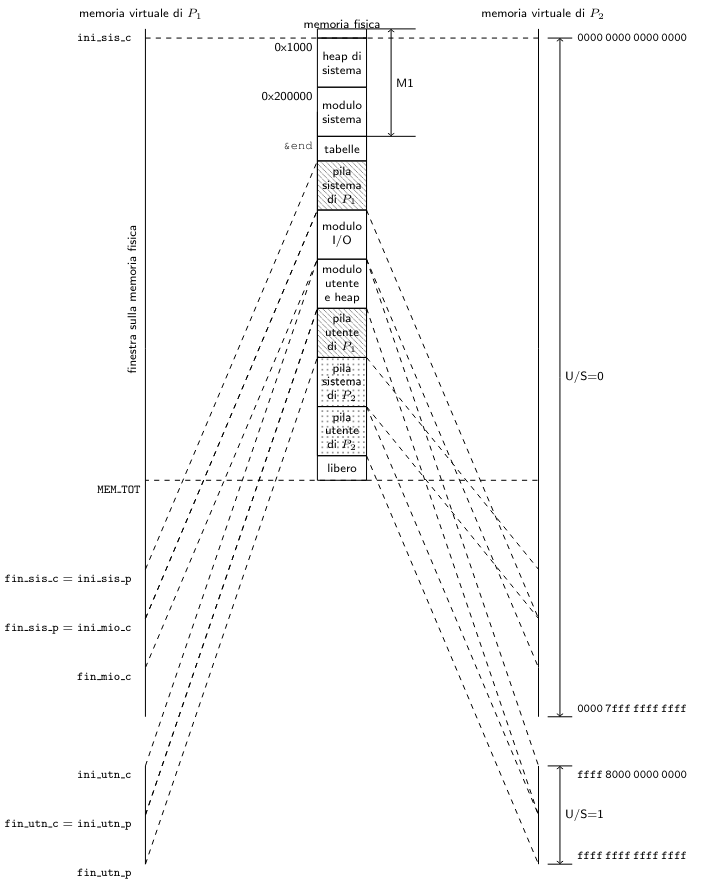
\includegraphics[scale=0.8]{../figures/mem_map.png}
\end{center}
in questo caso relativa ai trie di due processi, da cui notiamo ancora come la prima pagina non è tradotta, in quanto rappresenta l'area raggiungibile dai nullptr.
\end{minipage}

\par\bigskip

Facciamo allora alcune semplificazioni riguardo a questa struttura, in modo da avvicinarci ad un'implementazione effettiva:
\begin{itemize}
	\item Tutte le parti di livello più alte vengono create come multipli di 512 GiB, in modo che occupino intere entrate di livello 4;
	\item Le parti condivise sono \textit{"fisse"}, riferite da tabelle di livello 3 che vengono puntate nuovamente in ogni tabella di livello 4 che creiamo come radice degli alberi di traduzione di ogni processo (e che sono le stesse dell'albero di traduzione del nucleo). 
\end{itemize}

Vediamo che le tabelle di livello 3 della parte utente e sistema condivise si possono quindi creare una volta sola all'avvio del sistema (si dovrebbe ricaricare la parte codice dei processi nel caso di un sistema che carica software dal disco).
Questa allocazione viene fatta usando la \lstinline|map()| aiutata da \lstinline|alloca_frame()|, per ottenere memoria e disporre traduzioni per regioni di memoria di indirizzi prestabiliti.
Queste regioni seguono lo schema visto finora, che viene definito in codice come:
\begin{lstlisting}[language=C++, style=codestyle]	
#define I_SIS_C		0 	// prima entrata sistema/condivisa (inizio M1)
#define I_SIS_P		1		// prima entrata sistema/privata
#define I_MIO_C		2		// prima entrata modulo IO/condivisa
#define I_UTN_C   256	// prima entrata utente/condivisa (inizio M2)
#define I_UTN_P	  384	// prima entrata utente/privata

#define N_SIS_C		1		// numero entrate sistema/condivisa
#define N_SIS_P		1		// numero entrate sistema/privata
#define N_MIO_C		1		// numero entrate modulo IO/condivisa
#define N_UTN_C	  128	// numero entrate utente/convidisa
#define N_UTN_P	  128	// numero entrate utente/privata
\end{lstlisting}

Le uniche cose che vanno quindi create da zero ogni volta che si crea un processo sono la \textbf{pila sistema} in memoria sistema privata e la \textbf{pila utente} in memoria utente privata.

Avremo quindi che alla creazione di un nuovo processo dovremo creare una \textit{nuova} tabella di livello 4, che puntera alle tabelle di livello 3 delle parti condivise (memoria utente e sistema condivisa), già esistenti, e che creerà nuove tabelle di livello 3, e quindi di livello 2, ecc... per le parti private (pila utente e pila sistema).

\subsection{Creazione di processi in memoria}
Possiamo quindi vedere più nel dettaglio la creazione di processi, in particolare riguardo alla memoria e alle tabelle e traduzioni create.

\subsubsection{Albero di traduzione}
Abbiamo detto avevamo bisogno di creare nuove tabelle di livello 4 per ogni processo.
Facciamo questo come segue:
\begin{lstlisting}[language=C++, style=codestyle]	
des_proc* crea_processo(void f(natq), natq a, int prio, char liv) {
	[...]

	p->cr3 = alloca_tab(); // la nuova tabella di livello 4
	if (p->cr3 == 0)
		goto err_rel_id;
	init_root_tab(p->cr3);
	
	[...]
}
\end{lstlisting}
dove la \lstinline|init_root_tab()|, come avevamo detto, si limita a copiare le tabelle di livello 3 delle parti condivise:
\begin{lstlisting}[language=C++, style=codestyle]	
void init_root_tab(paddr dest) {
	// cr3 del processo corrente
	paddr pdir = esecuzione->cr3;

	// copia le tabelle di livello 3
	copy_des(pdir, dest, I_SIS_C, N_SIS_C);
	copy_des(pdir, dest, I_MIO_C, N_MIO_C);
	copy_des(pdir, dest, I_UTN_C, N_UTN_C);
}
\end{lstlisting}

Questa ha una duale, che semplicemente libera le entrate create:
\begin{lstlisting}[language=C++, style=codestyle]	
void clear_root_tab(paddr dest) {
	// eliminiamo le entrate create da init_root_tab()
	set_des(dest, I_SIS_C, N_SIS_C, 0);
	set_des(dest, I_MIO_C, N_MIO_C, 0);
	set_des(dest, I_UTN_C, N_UTN_C, 0);
}
\end{lstlisting}

\subsubsection{Pila}
Veniamo quindi all'inizializzazione della pila.
Questa si fa, sia per la pila utente che per la pila sistema, attraverso la \lstinline|crea_pila()|:
\begin{lstlisting}[language=C++, style=codestyle]	
bool crea_pila(paddr root_tab, vaddr bottom, natq size, natl liv)
{
	vaddr v = map(root_tab,
		bottom - size,
		bottom,
		BIT_RW | (liv == LIV_UTENTE ? BIT_US : 0),
		[](vaddr) { return alloca_frame(); });

	// caso di errore
	if (v != bottom) {
		unmap(root_tab, bottom - size, v,
			[](vaddr, paddr p, int) { rilascia_frame(p); });
		return false;
	}
	return true;
}
\end{lstlisting}
che ottiene una pila di una dimensione prestabilita allocando i frame necessari.

Questa ha ancora una duale, \lstinline|distruggi_pila()|:
\begin{lstlisting}[language=C++, style=codestyle]	
void distruggi_pila(paddr root_tab, vaddr bottom, natq size) {
	unmap(
		root_tab,
		bottom - size,
		bottom,
		[](vaddr, paddr p, int) { rilascia_frame(p); });
}
\end{lstlisting}
che si limita a liberare i frame usati.

Dal punto di vista della \lstinline|crea_processo()|, quindi, vogliamo prima inizializzare la pila sistema, e poi:
\begin{itemize}
	\item Se siamo in contesto utente:
		\begin{enumerate}
			\item Inizializzare la pila sistema;
			\item Creare la pila utente;
			\item Inizializzare la pila utente.
		\end{enumerate}
	\item Se invece siamo in contesto sistema, ci limitiamo ad inizializzare la pila sistema.
\end{itemize}

Questo in codice si traduce come:
\begin{lstlisting}[language=C++, style=codestyle]	
// creazione della pila sistema
static_assert(DIM_SYS_STACK > 0 && (DIM_SYS_STACK & 0xFFF) == 0);

// siamo in un altro processo, quindi dobbiamo accedere alla pila sistema tramite la finestra FM
pila_sistema = trasforma(p->cr3, fin_sis_p - 1) + 1;

// convertiamo a puntatore a natq, per accedervi piu' comodamente
pl = ptr_cast<natq>(pila_sistema);

if (liv == LIV_UTENTE) {
	// processo di livello utente
	// inizializzazione della pila sistema
	pl[-5] = int_cast<natq>(f);	    		// RIP (codice utente)
	pl[-4] = SEL_CODICE_UTENTE;	    		// CS (codice utente)
	pl[-3] = BIT_IF;	    	    				// RFLAGS
	pl[-2] = fin_utn_p - sizeof(natq);  // RSP
	pl[-1] = SEL_DATI_UTENTE;	    			// SS (pila utente)

	// eseguendo una IRET da questa situazione, il processo
	// passera' ad eseguire la prima istruzione della funzione f,
	// usando come pila la pila utente (al suo indirizzo virtuale)

	// creazione della pila utente
	static_assert(DIM_USR_STACK > 0 && (DIM_USR_STACK & 0xFFF) == 0);

	// inizialmente, il processo si trova a livello sistema, come
	// se avesse eseguito una istruzione INT, con la pila sistema
	// che contiene le 5 parole quadruple preparate precedentemente
	p->contesto[I_RSP] = fin_sis_p - 5 * sizeof(natq);

	p->livello = LIV_UTENTE;

	// dal momento che usiamo traduzioni diverse per le parti sistema/private
	// di tutti i processi, possiamo inizializzare p->punt_nucleo con un
	// indirizzo (virtuale) uguale per tutti i processi
	p->punt_nucleo = fin_sis_p;

	// tutti gli altri campi valgono 0
} else {
	// processo di livello sistema
	// inizializzazione della pila sistema
	pl[-6] = int_cast<natq>(f);				 // RIP (codice sistema)
	pl[-5] = SEL_CODICE_SISTEMA;  		 // CS (codice sistema)
	pl[-4] = BIT_IF;  	        			 // RFLAGS
	pl[-3] = fin_sis_p - sizeof(natq); // RSP
	pl[-2] = 0;			        					 // SS
	pl[-1] = 0;			        					 // ind. rit.

	// inizializzazione del descrittore di processo
	p->contesto[I_RSP] = fin_sis_p - 6 * sizeof(natq);

	p->livello = LIV_SISTEMA;

	// tutti gli altri campi valgono 0
}
\end{lstlisting}

\end{document}
